\documentclass[12pt, a4paper, twoside]{report}

\hbadness=10000
\hfuzz=50pt

%Publication list
\usepackage{bibentry}
\nobibliography*
%Spacing
\usepackage{setspace}
\doublespacing

%Abstract
\usepackage{abstract}
\renewcommand{\abstractnamefont}{\normalfont\bfseries\huge}

%Heading and footer
\usepackage{fancyhdr}
\setlength{\headheight}{15pt}
\pagestyle{fancy}
\renewcommand{\chaptermark}[1]{\markboth{#1}{}}
\renewcommand{\sectionmark}[1]{\markright{#1}{}}

 

\usepackage{graphicx}
\usepackage{subfig}
\usepackage{url}
\usepackage{listings}
\usepackage{multirow}
\usepackage{amsmath}
\usepackage{amsthm}
\usepackage{verbatim}
\usepackage{float}
\usepackage[plainpages=false, pdfpagelabels]{hyperref}
\usepackage{algorithm}
\usepackage{algorithmic}
\graphicspath{{./simulation/}{./figures/}{../figures/psware/}{../figures/shm/}{../simulation/psware/}{../Percom2011/simulation/}{../Percom2011/figures/}{../DCOSS2011/simulation/}{../DCOSS2011/figures/}}
\newcommand{\HRule}{\rule{\linewidth}{0.5mm}}
\newcommand{\figurecurrentwidth}{\includegraphics[width=.8\textwidth]}
\newcommand{\figurehalfwidth}{\includegraphics[width=.49\textwidth]}
%\newcommand{\figurecurrentwidth}{\includegraphics[width=.49\textwidth]}
%\newcommand{\figurehalfwidth}{\includegraphics[width=.24\textwidth]}

\lstset{
	basicstyle=\footnotesize\ttfamily,
	keywordstyle=\color{red},
	frame=lines,
	float,
	numbers=left,
	belowcaptionskip=6mm,
	xleftmargin=7mm,
	framexleftmargin=7mm,
	escapeinside={(*}{*)},
	tabsize=2,
	breaklines=true}
	
\newtheorem{theorem}{Theorem}
\renewcommand{\algorithmicrequire}{\textbf{Input:}}
\renewcommand{\algorithmicensure}{\textbf{Output:}} 
\pdfminorversion=9

\begin{document}
\fancyhf{}
\renewcommand{\headrulewidth}{0pt} % remove lines as well
\renewcommand{\footrulewidth}{0pt}
\pagenumbering{alph}
\begin{titlepage}
\begin{center}

% Upper part of the page

\includegraphics[width=0.15\textwidth]{./logo}\\[1cm]    

\textsc{\LARGE The Hong Kong Polytechnic University}\\[0.5cm]

\textsc{\Large Department of Computing}\\[0.5cm]

% Title
\HRule \\[0.4cm]
{ \LARGE \bfseries High Performance Publish / Subscribe Middleware for Wireless Sensor Network}\\[0.4cm]

\HRule \\[1cm]

% Author and supervisor
\begin{minipage}{0.4\textwidth}
\begin{flushleft} \large
\emph{Author:}\\
Steven \textsc{Lai}
\end{flushleft}
\end{minipage}
\begin{minipage}{0.4\textwidth}
\begin{flushright} \large
\emph{Supervisor:} \\
Dr.~Jiannong \textsc{Cao}
\end{flushright}
\end{minipage}

\vspace{2cm}
\textsc{\large A thesis submitted in partial fulfillment of the requirements for the degree of Doctor of Philosophy} 

\vfill

% Bottom of the page
{\large \today}

\end{center}

\end{titlepage}
\cleardoublepage
\vspace{5cm}

\begin{center}
\textsc{\LARGE Certificate of Originality}
%{\Large {CERTIFICATE OF ORIGINALITY}}
\end{center}

\vspace{2cm}
{\Large \bfseries I hereby declare that this thesis is my own work and that, to the best of my knowledge and belief, it reproduces no material previously published or written, nor material that has been accepted for the award of any other degree or diploma, except where due acknowledgment has been made in the text.}

\vfill

\begin{flushleft}
\includegraphics[width=0.25\textwidth]{./signature} \\
{\Large \bfseries \rule{8cm}{0.4pt} (Signed)}
\\[2cm]
{\Large Lai Yi} \\
{\Large \bfseries \rule{8cm}{0.4pt} (Name of student)}
\end{flushleft}

\cleardoublepage

\fancyhf{}
\fancyfoot[C]{\thepage}
\pagenumbering{roman}
\begin{abstract}
Event detection is an important topic in many WSN applications. Although there are several works on providing event-based services in WSN, most of them can only deal with primitive event types but cannot handle composite events very well. In general, a type-based event system may have primitive or composite event types. All event types are defined by specifying their attributes and filters. Then, individual events are detected and delivered according to such type information. Composite event types may be defined by combining multiple event types with operators. Due to the resource constraints in WSN, composite events are much more difficult to manage than primitive events. In this work, we introduce PSWare, a type-based publish / subscribe middleware for WSN that supports composite events. We describe our design for PSWare. PSWare has a flexible architecture where different composite event detection algorithms may be easily integrated.

On top of PSWare, we present TED (Type-based Event Detection), a novel distributed composite event detection algorithm. The essential idea of TED is event fusion, where some sensor nodes are selected as fusion points and component events are fused for the detection of a high level event. Event fusion with minimum energy cost is an NP-complete problem. Therefore, TED uses a number of heuristics with bounded performance.  

To further increase the performance of event detection, we design a clustering algorithm for PSWare for structural health monitoring applications (SHM). We formulate the problem and found it to be NP-complete so we propose heuristic centralized and distributed algorithms. In addition to SHM, We use PSWare to develop other real world WSN applications including intelligent transportation system (ITS) and in-door monitoring.

We evaluate our system from different aspects. We first evaluate TED, the most essential algorithm in our system. We analyze its performance and then carry out extensive simulations. Both analytical and simulation results show TED can save energy in event-based applications where primitive events occur in a higher frequency than composite events. Then we combine TED with PSWare and carried out some real world experiments. The results show that PSWare can offer reasonably simple API for the application developers to use while TED and our clustering algorithm can improve the underlying event detection performance. Compared with opportunistic approaches to event detection in these real applications, PSWare can reduce 40 - 50 \% of the energy cost.
\end{abstract} \cleardoublepage

\tableofcontents \cleardoublepage
\listoffigures \cleardoublepage
\listoftables \cleardoublepage

\pagenumbering{arabic}
\fancyhf{}
\fancyhead[RO]{\textit{\nouppercase{\leftmark}}}
\fancyhead[LO]{\textit{\nouppercase{\chaptername \thechapter}}}
\fancyhead[CE]{A Thesis Submitted by Steven Lai}
\fancyfoot[C]{\thepage}

\chapter{Introduction}
\section{Overview}
\label{sec:introduction}
Development in wireless communication and electronics has made it possible to create low-cost, low-power wireless sensor nodes. Each sensor node usually contains a wireless transceiver, a micro processing unit and a number of sensors. The sensor nodes can collect data and do some simple processing locally, and can communicate with each other to form an ad hoc wireless sensor network (WSN) \cite{aky:survey}. A WSN is usually self-organized and self-maintained without any human intervention. Wireless sensor networks have been used in various application areas such as smart building \cite{lynch:shm}, wild environment monitoring \cite{wsnhabitat}, intelligent transportation systems \cite{klein:its}, battle surveillance \cite{wsntracking} and healthcare \cite{lo:ban}. 

While WSN has a wide range of applications, programming sensor networks is a challenging because different from programming in the traditional environment. WSN imposes a lot of constraints such as limited computational power, less memory and unreliable communication. Application developers need to not only understand the requirements for the specific application domain but also take into consideration of the characteristics of WSN. In this research work, we propose PSWare, a publish/subscribe (pub/sub) middleware for WSN which eases the development of WSN applications. Our middleware uses a pub/sub programming paradigm for the application programmer to subscribe application specific events. It provides an easy-to-use Event Definition Language (EDL) to allow the application developers to define composite events while uses a flexible architecture so that different domain-specific event processing algorithms can be easily integrated into the middleware.

\subsection{Motivation}
Despite the large variety of WSN applications, many of them are essentially event-based. In applications such as intelligent transportation systems \cite{klein:its}, smart buildings \cite{lynch:shm} and healthcare \cite{lo:ban}, the events sensor nodes detect events which reflect the environmental changes and the systems respond to these events accordingly. Events may be primitive or composite. Primitive events (e.g. when the temperature exceeds certain threshold) can be detected by a single sensor node without having to cooperate with others. On the other hand, \emph{composite events} consist of multiple primitive events. They reflect a serial of environmental changes with spatial and temporal relations among them and must be detected collaboratively by different sensor nodes.

Because of the common requirements and challenges for composite event subscription and detection, it is more desirable to have a generic middleware layer to handle composite events instead of reinventing the wheel and implementing application-specific event processing mechanisms. In addition, the middleware should be flexible enough so that different event processing algorithms for different application domains can be easily integrated. In summary, the middleware should achieve the following design goals:
\begin{enumerate}
\item \emph{Event abstraction}: since composite events are collaboratively processed by different sensor nodes in the network, they introduce extra complexity because of the resource constraints and unreliable communication. A middleware framework providing high level event abstraction is needed to ease the application development.
\item \emph{Re-usability and flexibility}: different applications may share certain common modules during event processing. They may also have other different modules. A middleware framework can help so that common modules may be used and different modules may be replaced without affecting others.
\end{enumerate}

\subsection{Issues}
In this research, we address the essential issues of designing and developing PSWare. On the highest level, an event description language is provided to allow users to describe composite event relationships. On the lowest level, a runtime environment is necessary on each sensor nodes so that they could understand and execute the event processing algorithms translated from the high-level EDL. More specifically, we need to address the following research/engineering issues to make our middleware work.

\begin{itemize}
\item	\emph{Event definition language}: we need to provide an event description language which is powerful yet easy to use.
\item	\emph{Event definition language compiler}: a compiler is essential to translate the programs written in our high-level language into a low-level language understandable by the sensor nodes. The compiler must be smart enough to extract the semantic meanings from the program and do some optimization.
\item	\emph{Runtime environment support}: the middleware running on each sensor node should provide a runtime environment to execute the compiled programs.
\item	\emph{Subscription propagation}: after the program written in EDL is compiled, the subscription should be intelligently disseminated into the network. If the subscription is too big, it may need to be divided into small ones. Furthermore, only related sensor nodes need to be updated.
\item	\emph{Event detection}: we need to design efficient protocol for the sensor nodes to cooperate with each other to detect composite events.
\item	\emph{Event delivery}: after the subscribed the events have been detected, we need energy-efficient routing protocols so that the detected events will be delivered at the minimum cost.
\end{itemize}
\section{Background}
\label{sec:background}
\begin{comment}
We first briefly overview the issues in event subscription and event detection.
\end{comment}
\subsection{Event Types and Subscriptions}
Each event contains a list of attributes which are the actual data obtained from the sensors. Users can subscribe events with subscriptions which specify event types and event filters. Different event types can have relations among each other. The relations may also be expressed as special type of filters that operate on multiple event types. Listing \ref{prog:compositeExample} shows how a composite event type is defined \cite{lai:psware}. The event type 'CompTemp' requires two sub-events of type 'AvgTemp'. The two sub-events must satisfy certain temporal constraints in order to indicate the occurrence of the composite event.
\begin{lstlisting}[caption=Example of a composite event, label=prog:compositeExample]
Event CompTemp {
} on {
    AvgTemp e1 and
    AvgTemp e2
} where {
    e2.time-e1.time=600
}
\end{lstlisting}
\begin{comment}
Mathematically, event types together with their relations can be represented by a directed acyclic graph, where each node represents an event and each edge represents a relation. The nodes with 0 indegree represent primitive event types which are the events that can be directly obtained from individual sensor nodes. The rest of the nodes represent composite event types. The event type which has 0 outdegree is the subscribed event type.
\end{comment}
Once the subscriptions are defined, it will be disseminated into the network so that sensor nodes start to detect the corresponding events. In a pub/sub system, if an event is detected to match the subscribed event type, it will be delivered to the sink to notify the subscriber.

\subsection{Type-based Event Detection}
In our approach to event detection, we make use of some special nodes called event fusion points. These nodes take the responsibility of composite event detection. The event fusion points may have some extra capabilities in terms of processing power or storage though it's not compulsory. For each event fusion point, it has an event detection framework as shown in Figure \ref{fig:eventdetectionframework2}. In such a framework, events are stored in a buffer and associated with types. Each event type has a corresponding filter so that the fusion points can decide if the event occurs or not. The event filters consist of some predicates on the event attributes.
Event detection based on our model involves three steps:
\begin{enumerate}
\item Detect an event either locally or receive an event from other nodes. Then store it in the buffer. 
\item Look up for the corresponding filter for that event.
\item Evaluate the event against the filter.
\item If the event is evaluated to have happened, make a decision on where to send the event.
\end{enumerate}

\begin{figure}
\centering
\figurecurrentwidth{eventdetectionframework2}
\caption{Type-based event detection framework}
\label{fig:eventdetectionframework2}
\end{figure}

The event detection framework in Figure \ref{fig:eventdetectionframework2} is essentially type-based event detection because the predicates are grouped according to the event types. In addition, compared with topic or content-based approach, type-based event detection is more suitable for WSN-based applications. Because of the resource constraints in WSNs, it is usually not efficient to send all the primitive events to the sink node for centralized event detection. Instead, events should be detected in-network if possible. Composite events in WSNs may have multiple levels and higher level events cannot be detected until its sub-events have been detected. Therefore, in-network event detection must take the event types into consideration in order to detect the events.  

\begin{comment}
Second, pure topic based event detection may not be suitable for WSNs because many WSNs require events that have different data types or topics. For example the detection of fire may require both temperature and light event topics. Without considering event types, it is very difficult to do in-network composite events detection just based on the event topics. Third, similar to topic based event detection, content based event detection without considering event types can only filter the primitive events and may not be efficient if the lower-level events occur with a much higher frequency than composite events.
\end{comment}
\cleardoublepage

\begin{figure}
\centering
\figurecurrentwidth{psware-architecture}
\caption{Event processing in PSWare}
\label{fig:psware-architecture}
\end{figure}

\section{Composite Event Processing in PSWare}
\label{sec:design}
In this section, we discuss how PSWare is designed to support composite event. The overall work flow of event processing in PSWare is shown in Figure \ref{fig:psware-architecture}. To use the middleware, applications developers will first define event types according to the application requirements. The subscription will then be compiled and processed by the EDL compiler and be disseminated into the network. When the events are detected by the sensor nodes, they will be delivered to the application.

\subsection{Event Specification}
\begin{figure}
\centering
\figurecurrentwidth{edlcompiler}
\caption{PSWare-EDL compiler structure}
\label{fig:edlcompiler}
\end{figure}

EDL is used for specifying events in PSWare. For each EDL script, it contains one or more event definition and one subscribing statement. Formally, the BNF of the subscription is defined in Listing \ref{lst:BNFSubscription}.

\begin{lstlisting}[caption=BNF (simplified) of subscription, label=lst:BNFSubscription]
subscription -> event_declarations subscribe_statement
event_declarations -> event_declaration | event_declarations event_declaration
subscribe_statement -> SUBSCRIBE IDENTIFIER SEMICOLON
\end{lstlisting}

The subscribe statement simply uses the keyword 'subscribe' followed the event type name needed by the application. Each event type declaration can have up to three parts: the event body, the where clause and the on clause. The event body defines the attributes of the events. The on clause are used to specify the sub-events used by a composite event. The where clause defines the filter of the corresponding event type. Formally, the BNF of event type is defined in Listing \ref{lst:BNFEvent}

\begin{lstlisting}[caption=BNF (simplified) of event type, label=lst:BNFEvent]
event_declaration -> EVENT IDENTIFIER event_body on_clause_opt where_clause_opt
event_body -> { field_declarations_opt }
on_clause -> ON { subevent_declarations_opt }
where_clause -> WHERE { conditional_expression }
\end{lstlisting}

The on clause and the where clause are both optional in case if the event is primitive or does not have a filter. The on clause looks similar to the field declaration except sub-events instead of fields are declared. This is done for a clear code presentation and easier type checking. The where clause simply consists of conditional expressions so that the filters may be defined by specifying the operators.

\begin{comment}
A simple example of using EDL is shown in Listing \ref{lst:originaledl}. In this example, two events, 'SimpleEvent' and 'CompEvent' are defined. 'SimpleEvent' is a primitive event which occurs when the detected temperature reading is above certain threshold. 'CompEvent' is a composite event that is based on two events of 'SimpleEvent' and their time must satisfy a certain condition in order to indicate the occurrence of 'CompEvent'.
\begin{lstlisting}[caption=A simple EDL program, label=lst:originaledl]
Event SimpleEvent {
	int temp=System.temp;
	int id=System.id;
	int time=System.time;
} where {
	temp > 30
}
Event CompEvent {
} on {
	SimpleEvent e1 and
	SimpleEvent e2
} where {
	e2.time-e1.time=600
}
\end{lstlisting}
\end{comment}

The EDL-based subscription will be processed by our EDL compiler. The output of the compiler has two parts as shown in Figure \ref{fig:edlcompiler}. The first part is the byte codes which will be executed by individual sensors to detect events. The format and the organization of the byte codes are closely related to the event processing framework and customization of PSWare. We will go through these topics in the following sections.

\begin{figure}
\centering
\figurecurrentwidth{edlcompiler-flow}
\caption{EDL compiler flow}
\label{fig:edlcompiler-flow}
\end{figure}

The second part, the event receiving module is the implementation of the event notifier as discussed in Section \ref{sec:model}. As shown in Figure \ref{fig:edlcompiler-flow}, The EDL compiler will execute the following steps in order to generate the byte codes and event receiving module:
\begin{enumerate}
\item Parse the EDL script and generate the corresponding syntax tree and symbol table.
\item Generate the byte codes based on the syntax tree and symbol table.
\item Create the event receiving module based on the symbol table.
\end{enumerate}

\subsection{Runtime Environment for Event Detection}
The byte codes generated by the compiler can be further divided into three parts: event meta data, event filters and event matcher. These components implements the programming interface discussed in Listing \ref{lst:pswareAPI} and \ref{lst:pswareEventMatcher}. Event meta data contains the description of the event types such as event type ID, event size and the individual attributes for each event. Event filters are the constraints defined for each event type. Event matcher schedules the execution for event detection according to the subscription and event relations.

The runtime environment on each sensor node is similar to the VM-based approach \cite{mate} in the sense that the subscriptions are broken down into some basic operations called instructions. Such design choice is for extensibility so that new features can be added more easily by adding new instructions. In addition to the VM-based runtime environment, each sensor node has an event buffer where the detected events can be stored for composite event detection.

\begin{figure}
\centering
\figurecurrentwidth{eventdetectionframework2}
\caption{PSWare runtime environment}
\label{fig:eventdetectionframework2}
\end{figure}
The essential operations for our runtime environment is shown in Figure \ref{fig:eventdetectionframework2}. In this environment, the event matcher will first fetch the events from the event buffer and then evaluate them against the corresponding filters. If the event has been detected, then it will be transmitted over the network. Formally, the procedure of the event matcher can be shown in Procedure \ref{algo:eventmatcher} with some notations defined as:
\begin{itemize}
\item Event types: \(E=\{e_1, e_2 \cdots \}\)
\item For each \(e_n\in E\), its filter is: \(e_n\rightarrow filter\)
\item For each \(e_n\in E\), it has a set of events \(E_n=\{e_n^1, e_n^2 \cdots \}\) stored in the buffer.
\end{itemize}

\begin{algorithm}
\begin{algorithmic}
\REQUIRE \(E\)
	\FORALL {\(e_n\in E\)}
		\FORALL {\(e_n^i\in E_n\)}
			\IF {\(e_n\) is primitive}
				\STATE result = evaluate\_primitive (\(e_n^i\))
				\IF {result == True}
					\STATE eventMatched(\(e_n^i\))
					\IF {\(e_n\) is subscribed}
						\STATE deliver(\(e_n^i\))
					\ELSE
						\STATE forward(\(e_n^i\))
					\ENDIF
				\ENDIF
			\ELSE
				\STATE \(e_{sub} = \emptyset \)
				\FORALL {subevents \(e_m\) for \(e_n\)}
					\STATE \(e_{sub} = e_{sub}\bigcup selectSubevent (e_n, e_m)\)
				\ENDFOR
				\FORALL {subevents \(e_m\) for \(e_{sub}\)}
					\STATE evaluate\_composite(\(e_n^i\), \(e_m\), \(\cdots \))
				\ENDFOR
			\ENDIF
		\ENDFOR
	\ENDFOR
\end{algorithmic}
\caption{Procedure of the event matcher}
\label{algo:eventmatcher}
\end{algorithm}

There are several keys in the procedure. First, when the event matcher picks up the events of type \(e_n\) from the event buffer, it may use application specific mechanisms to pick up the desired events instead of trying all the possible combinations. Second, the 'deliver()' and the 'forward()' function are used to deliver the subscribed events or forward the events so that composite events may be detected. These two functions may also be application dependent to achieve high energy efficiency.

\begin{comment}
Figure \ref{fig:psware-interaction-simple} illustrates how different components in the middleware system interact with each other.

\begin{figure}
\centering
\figurecurrentwidth{psware-interaction-simple}
\caption{PSWare-E components interaction}
\label{fig:psware-interaction-simple}
\end{figure}
\subsection{PSWare Customization}
\end{comment}

Finally, it is necessary to mention the 'SystemEvent'. This module acts as the device driver for PSWare. It defines the sampling rate and a primitive event. All the fields of other events are obtained from 'System'. The module needs to implement three interfaces: StdControl, SystemClock and SystemEvent as shown in Listing \ref{lst:systemEvent}. StdControl is a module for initialization purpose. SystemClock defines the sampling frequency. SystemEvent is used to obtain the pointer to the 'System' event.

\begin{lstlisting}[caption=API of the 'System' event, label=lst:systemEvent]
module SystemEventM {
	provides {
		interface StdControl;
		interface SystemEvent;
		interface SystemClock;
	}
}
interface SystemEvent {
	command EventInstanceInfo * get();
}
\end{lstlisting}

The 'SystemEvent' is there so that needs to be implemented by the middleware developers as the  Once the 'System' event is defined, the application developers can further define their own functions for event delivery and event forwarding. We will show some examples in the next section. 
\section{EDL and Its Compiler}
Like other type-based pub/sub systems, the programming model provided by PSWare is similar to object-oriented model where the events are treated like objects. In such kind of model, developers express the application requirements in terms of the events to be detected from the WSN as shown in Figure \ref{fig:eventprogramming}.

\begin{figure}
\centering
\figurecurrentwidth{eventprogramming}
\caption{Event-oriented Programming Model}
\label{fig:eventprogramming}
\end{figure}

\subsection{Event Definition Language}
EDL uses familiar SQL-like syntax and allows the users to reuse and combine different events and create new composite events. The subscription contains one or more event definition and one subscribing statement. Formally, the BNF of the subscription is defined in Listing \ref{lst:BNFSubscription}.

\begin{lstlisting}[caption=BNF (simplified) of subscription, label=lst:BNFSubscription]
subscription -> event_declarations subscribe_statement
event_declarations -> event_declaration | event_declarations event_declaration
subscribe_statement -> SUBSCRIBE IDENTIFIER SEMICOLON
\end{lstlisting}

The subscribe statement simply uses the keyword 'subscribe' followed the event type name needed by the application. Each event type declaration can have up to three parts: the event body, the where clause and the on clause. The event body defines the attributes of the events. The on clause are used to specify the sub-events used by a composite event. The where clause defines the filter of the corresponding event type. Formally, the BNF of event type is defined in Listing \ref{lst:BNFEvent}

\begin{lstlisting}[caption=BNF (simplified) of event type, label=lst:BNFEvent]
event_declaration -> EVENT IDENTIFIER event_body on_clause_opt where_clause_opt
event_body -> { field_declarations_opt }
on_clause -> ON { subevent_declarations_opt }
where_clause -> WHERE { conditional_expression }
\end{lstlisting}

The on clause and the where clause are both optional in case if the event is primitive or doesn't have a filter. The on clause looks similar to the field declaration except sub-events instead of fields are declared. This is done for a clear code presentation and easier type checking. The where clause simply consists of conditional expressions so that the filters may be defined by specifying the operators.

A simple example of using EDL is shown in Listing \ref{lst:EDLExample}. In this example, two events, 'SimpleEvent' and 'CompEvent' are defined. 'SimpleEvent' is a primitive event which occurs when the detected temperature reading is above certain threshold. 'CompEvent' is a composite event that is based on two events of 'SimpleEvent' and their time must satisfy a certain condition in order to indicate the occurrence of 'CompEvent'.
\begin{lstlisting}[caption=A simple EDL program, label=lst:EDLExample]
Event SimpleEvent {
	int temp=System.temp;
	int id=System.id;
	int time=System.time;
} where {
	temp > 30
}
Event CompEvent {
} on {
	SimpleEvent e1 and
	SimpleEvent e2
} where {
	e2.time-e1.time=600
}
\end{lstlisting}

\subsection{EDL Compiler}
The EDL-based subscription will be processed by our EDL compiler. The output of the compiler has two parts as shown in Figure \ref{fig:edlcompiler}. The first part is the byte codes which will be executed by individual sensors to detect events. We will discuss how the sensor nodes will execute the byte codes in the next section. The second part is the event receiving module. This module is responsible for receiving and interpreting the events delivered from WSN and notify the application layer if the subscribed events are delivered.

\begin{figure}
\centering
\figurecurrentwidth{edlcompiler}
\caption{EDL compiler structure}
\label{fig:edlcompiler}
\end{figure}

Internally, the compiler has the structure shown in Figure \ref{fig:compilerinternal}. The program written in EDL is firstly processed by the lexer and parser to generate a syntax tree. Then type check will be performed to add necessary attributes to the tree. Then the tree will be passed to the backend code generator to generate target codes.

\begin{figure}
\centering
\figurecurrentwidth{compilerinternal}
\caption{EDL compiler internal}
\label{fig:compilerinternal}
\end{figure}

The key step of the compiler is to transform EDL programs into trees. For example, the BNF for event declaration is shown as Listing \ref{lst:eventDefinitionBNF}. The corresponding tree will look like the one in Figure \ref{fig:eventDefinitionTree}. The circles represent the exact tree nodes while the boxes are the attributes.

\begin{lstlisting}[caption=BNF for event definition, label=lst:eventDefinitionBNF]
event_declaration ::= EVENT IDENTIFIER:id event_body:b on_clause_opt:o filter_body_opt:f;
event_body ::= LBRACE field_declarations_opt:f RBRACE
on_clause ::= ON LBRACE field_declarations_opt:f RBRACE	;
filter_body ::=	WHERE LBRACE conditional_expression:e RBRACE;
\end{lstlisting}

\begin{figure}
\centering
\figurecurrentwidth{eventDefinitionTree}
\caption{Syntax tree for event definition}
\label{fig:eventDefinitionTree}
\end{figure}
\section{Event Detection Framework}
The byte codes generated by the compiler can be further divided into three parts: event meta data, event filters and event matcher. Event meta data contains the description of the event types such as event type ID, event size and the individual attributes for each event. Event filters are the constraints defined for each event type. Event matcher schedules the execution for event detection according to the subscription and event relations.

\subsection{The Runtime Environment}
The runtime environment on each sensor node is similar to the VM-based approach \cite{mate} in the sense that the subscriptions are broken down into some basic operations. Such design choice is for the extensibility of the middleware so that different event detection mechanisms may be easily implemented through the operations. In addition to the VM-based runtime environment, as shown in Figure \ref{fig:pswarevm}, each sensor node has an event buffer where the detected events may be stored for composite event detection.

\begin{figure}
\centering
\figurecurrentwidth{pswarevm}
\caption{PSWare runtime environment}
\label{fig:pswarevm}
\end{figure}

The essential operations for our event detection framework is shown in Figure \ref{fig:eventdetectionframework2}. In this framework, the event matcher will first fetch the events from the event buffer and then evaluate them against the corresponding filters. If the event has been detected, then it will be transmitted over the network. Formally, the procedure of the event matcher can be shown in Algorithm \ref{algo:eventMatcher} with some notations defined as:
\begin{itemize}
\item Event types: \(E=\{e_1, e_2 \cdots \}\)
\item For each \(e_n\in E\), its filter is: \(e_n\rightarrow filter\)
\item For each \(e_n\in E\), it has a set of events \(E_n=\{e_n^1, e_n^2 \cdots \}\) stored in the buffer.
\end{itemize}

\begin{figure}
\centering
\figurecurrentwidth{eventdetectionframework2}
\caption{Event detection framework}
\label{fig:eventdetectionframework2}
\end{figure}

\begin{algorithm}
\begin{algorithmic}[1]
\REQUIRE \(E\)
	\FORALL {\(e_n\in E\)}
		\FORALL {\(e_n^i\in E_n\)}
			\IF {\(e_n\) is primitive}
				\STATE result = evaluate\_primitive (\(e_n^i\))
				\IF {result == True}
					\IF {\(e_n\) is subscribed}
						\STATE deliver(\(e_n^i\))
					\ELSE
						\STATE forward(\(e_n^i\))
					\ENDIF
				\ENDIF
			\ELSE
				\FORALL {subevents \(e_m\) for \(e_n\)}
					\STATE evaluate\_composite(\(e_n^i\), \(e_m\), \(\cdots \))
				\ENDFOR
			\ENDIF
		\ENDFOR
	\ENDFOR
\end{algorithmic}
\caption{Procedure of the event matcher}
\label{algo:eventMatcher}
\end{algorithm}

There are several keys in the procedure. First, when the event matcher picks up the events of type \(e_n\) from the event buffer, it may use application specific mechanisms to pick up the desired events instead of trying all the possible combinations. Second, the 'deliver()' and the 'forward()' function are used to deliver the subscribed events or forward the events so that composite events may be detected. These two functions may also be application dependent to achieve high energy efficiency.

Figure \ref{fig:psware-interaction-simple} illustrates how different components in the middleware system interact with each other.

\begin{figure*}
\centering
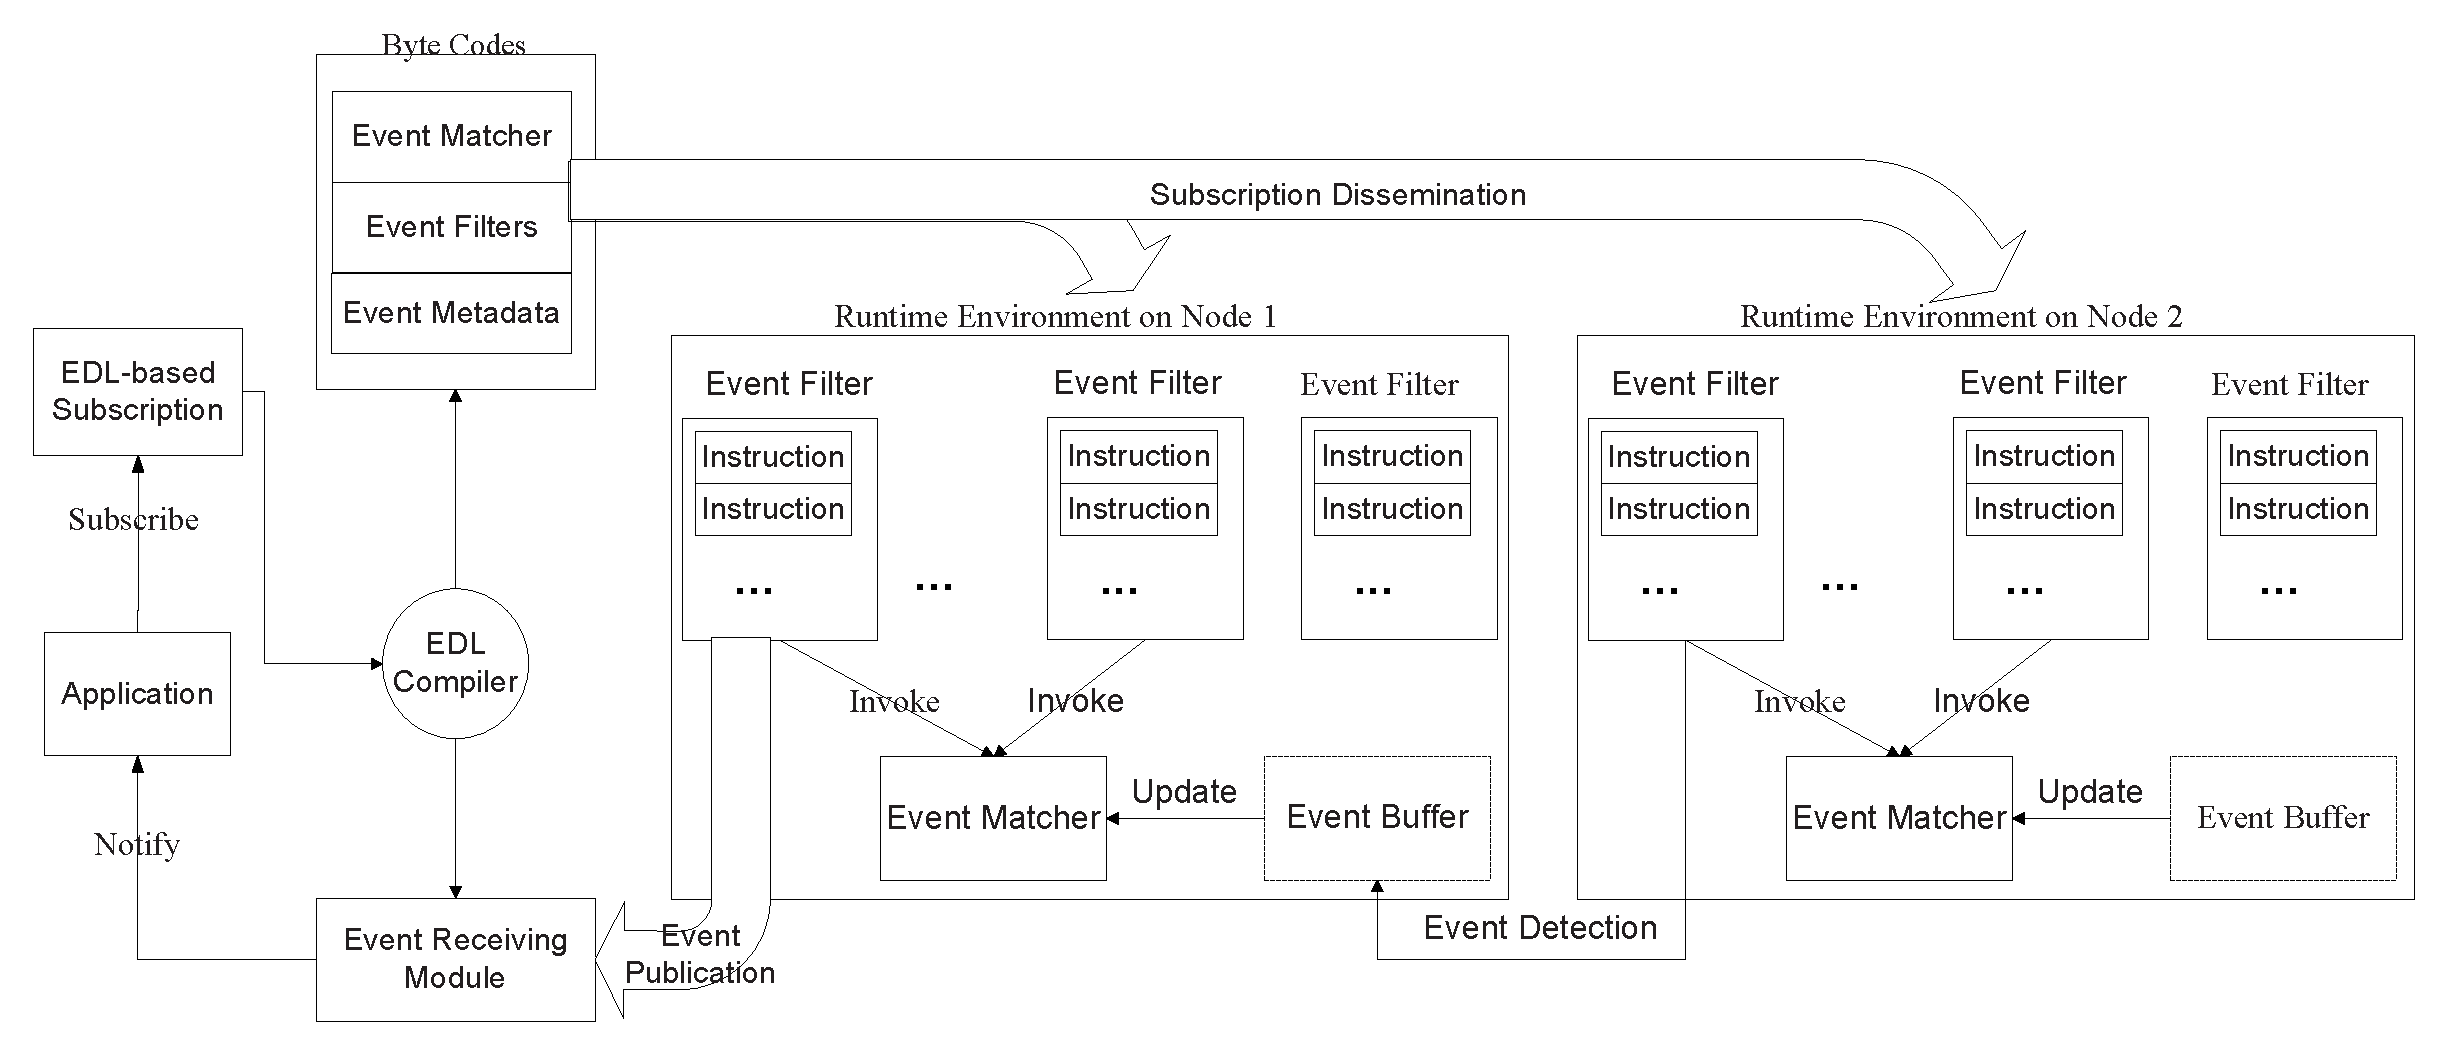
\includegraphics[width=\textwidth]{psware-interaction-simple}
\caption{PSWare components interaction}
\label{fig:psware-interaction-simple}
\end{figure*}
\subsection{Basic Instructions}
The design of our event detection framework makes it very suitable to be implemented using a VM-based architecture and this is how we implemented it in the bytecodes for the sensor nodes. Our VM-based runtime environment is based on Mat\'{e} \cite{mate}. It uses stack-based instructions which allow compact code size. We choose a VM-based runtime environment because it is more flexible in terms of interfacing with the EDL compiler and introducing new modules. Apart from the existing instructions which are already available in Mat\'{e}, we have mainly added the following instructions used specifically for event detection.
\begin{itemize}
	\item \emph{OPref}: whenever an event \(e\) is being evaluated, this instruction is invoked to obtain an instance of such event.
	\item \emph{OPoffset}: this instruction is involved right after the 'ref' instruction, in order to access individual attributes of the event instance.
	\item \emph{OPset}: if the attributes of an event need to be changed, this instruction will be used.
	\item \emph{OPget}: the 'get' instruction does the opposite of 'set' instruction. It will simply retrieve content of a specific attribute in an event.
	\item \emph{OPcreate}: is used to create a new instance of an event.
	\item \emph{OPeval}: is used to determine if an event happens or not.
\end{itemize}
For a complete list of all the instructions, please refer to Appendix \ref{appendix:isa} We give a simple example how EDL can be translated to the lower level runtime instruction sets. Consider a very simple event shown in Listing \ref{lst:originaledl}. The event will occur when the temperature reading on sensor node 5 is above 30. It's corresponding program for the VM is shown in Listing \ref{lst:translatededl}. Since 'SimpleEvent' is a primitive event, so every time it is being detected, a new instance of the event will be created. The ID of 'SimpleEvent' is \(1\). Here we also have another event called 'System' which is a built-in event provided by EDL as a place where all the sensor data can be obtained. The 'System' event has a default ID of \(0\) as shown on Line \ref{line:systemevent} in Listing \ref{lst:translatededl}. Each attributes in the event will have it's unique ID. In the example, the ID of the attribute is calculated simply by the order of their appearance. For example, temperature has the ID of \(0\) on Line \ref{line:systemevent}.

\begin{lstlisting}[caption=Original EDL program, label=lst:originaledl]
Event SimpleEvent {
	int temp=System.temp;
	int id=System.id;
} where {
	temp > 30 and
	id == 5
}
\end{lstlisting}
\begin{lstlisting}[caption=Translated EDL program, label=lst:translatededl]
alloc 1
ref 0 (*\label{line:systemevent}*)
offset 0
ref 1
offset 0
set
ref 0
offset 1
ref 1
offset 1 (*\label{line:idattr}*)
set
ref 1
offset 1
get
push 30
gt
ref 1
offset 1
get
push 5
eq
and
eval
\end{lstlisting}

\subsection{Customizing PSWare}
The event detection framework of PSWare is developed using NesC. As discussed in the previous section, many of the operations in PSWare can be defined according to applications. In this section, we describe how we can customize PSWare.

The first step is to implement a special module which acts like a device driver for PSWare. This module defines the sampling rate and a primitive event called 'System'. All the fields of other events are obtained from 'System'. The module needs to implement three interfaces: StdControl, SystemClock and SystemEvent as shown in Listing \ref{lst:systemEvent}. StdControl is a module for initialization purpose. SystemClock defines the sampling frequency. SystemEvent is used to obtain the pointer to the 'System' event.

\begin{lstlisting}[caption=API of the 'System' event, label=lst:systemEvent]
module SystemEventM {
	provides {
		interface StdControl;
		interface SystemEvent;
		interface SystemClock;
	}
}
interface SystemEvent {
	command EventInstanceInfo * get();
}
\end{lstlisting}

Once the 'System' event is defined, the application developers can further define their own functions for event delivery and event forwarding. We will show some examples in the next section. In addition, they can make use of the API provided by PSWare as shown in Listing \ref{lst:pswareAPI}.

\begin{lstlisting}[caption=API provided by PSWare, label=lst:pswareAPI]
interface EventMeta {
	command EventMetaInfo * getEventMeta(uint8_t subID);
	command bool isSubscribed(uint8_t subID);
	command bool isComposite(uint8_t subID);
	command bool isAggregate(uint8_t subID);
}
interface EventInstance {
	command EventInstanceInfo * createEvent(uint8_t subID);
	command int instanceAmount(uint8_t subID);
	command void deleteEvent(uint8_t subID, uint8_t instanceID);
	command EventInstanceInfo * getEventInstance(uint8_t subID, int idx);
}
interface EventMatcher {
	command bool selectSubevent(EventInstanceInfo * composite, EventInstanceInfo * subevent);
	command result_t eventDetected(uint8_t subID, uint8_t instanceID, bool detectionResult);
	command result_t eventDelivery(uint8_t subID, uint8_t instanceID, bool detectionResult);
}
\end{lstlisting}

These API provides the necessary functionalities for accessing modules such as event meta data or the event buffer (as in EventInstance). To implement application specific event detection mechanisms, application developers simply need to override the commands provided in the EventMatcher interface. The 'selectSubevent()' command is used to determine if a sub-event (in the parameter subevent) should be used to detect a composite event (in the parameter composite).
\section{Complete List of the Instructions for EDF}
\label{appendix:isa}
In this section, we show the complete list of instructions currently used by our Event Detection Framework (EDF). We also briefly describe the function and the usage of each instruction.

\subsection{Basic Instructions}
The basic instruction deals with the most fundamental operations. Since the instruction uses a stack-based architecture in order to reduce the code size, most of the instructions that fall into this category deal with the operations related stacks.
\begin{itemize}
\item \emph{OPpush}: this instruction is used to push an operand to the top of the stack.
\item \emph{OPpop}: this instruction is used to pop and discard an operand from the top of the stack.
\item \emph{OPcopy}: duplicates the top operand of the stack
\item \emph{OPhalt}: once this instruction is reached, the VM will stop execution.
\end{itemize}

\subsection{Operators}
Basic mathematical operators:
\begin{itemize}
\item \emph{OPadd}: pops two operands off the top of the stack, add them together and push the result back to the top of the stack.
\item \emph{OPmult}: pops two operands off the top of the stack, multiply them together and push the result back to the top of the stack.
\item \emph{OPsub}: pops two operands off the top of the stack, subtract the first popped number by the second one and push the result back to the top of the stack.
\item \emph{OPdiv}: pops two operands off the top of the stack, divide the first popped number by the second one and push the result back to the top of the stack.
\item \emph{OPmod}: pops two operands off the top of the stack, divide the first popped number by the second one and push the remainder back to the top of the stack.
\item \emph{OPinv}: pops one operand (n) off the top of the stack, calculate its inverse (-n) and push the result back.
\end{itemize}

Logical operators:
\begin{itemize}
\item \emph{OPand}: pops two operands off the top of the stack, calculate the logical and of them and push the result back to the top of the stack.
\item \emph{OPor}: pops two operands off the top of the stack, calculate the logical or of them and push the result back to the top of the stack.
\item \emph{OPxor}: pops two operands off the top of the stack, calculate the exclusive or of them and push the result back to the top of the stack.
\item \emph{OPnot}: pops one operand off the top of the stack, calculate the logical not of it and push the result back to the top of the stack.
\end{itemize}

Relational operators:
\begin{itemize}
\item \emph{OPeq}: pops two operands off the top of the stack, if the two operands are equal, push 1 to stack. Otherwise, push 0 to stack.
\item \emph{OPneq}: pops two operands off the top of the stack, if the two operands are equal, push 0 to stack. Otherwise, push 1 to stack.
\item \emph{OPgt}: pops two operands off the top of the stack, if the first operand is greater than the second one, push 0 to stack. Otherwise, push 1 to stack.
\item \emph{OPgte}: pops two operands off the top of the stack, if the first operand is greater than or equal to the second one, push 0 to stack. Otherwise, push 1 to stack.
\item \emph{OPlt}: pops two operands off the top of the stack, if the first operand is less than the second one, push 0 to stack. Otherwise, push 1 to stack.
\item \emph{OPlte}: pops two operands off the top of the stack, if the first operand is less than or equal to the second one, push 0 to stack. Otherwise, push 1 to stack.
\end{itemize}

Bitwise operators:
\begin{itemize}
\item \emph{OPshiftl}: pops two operands off the top of the stack, left shift the first popped number by the second one and push the result back to the top of the stack.
\item \emph{OPshiftr}: pops two operands off the top of the stack, right shift the first popped number by the second one and push the result back to the top of the stack.
\item \emph{OPland}: pops two operands off the top of the stack, calculate the bitwise and of them and push the result back to the top of the stack.
\item \emph{OPlor}: pops two operands off the top of the stack, calculate the bitwise or of them and push the result back to the top of the stack.
\item \emph{OPxor}: pops two operands off the top of the stack, calculate the bitwise exclusive or of them and push the result back to the top of the stack.
\item \emph{OPlnot}: pops one operand off the top of the stack, calculate its complement and push the result back to the top of the stack.
\end{itemize}

\subsection{Event-related Instructions}
\begin{itemize}
\item \emph{OPref}: whenever an event \(e\) is being evaluated, this instruction is invoked to obtain an instance of such event.
\item \emph{OPoffset}: this instruction is involved right after the 'ref' instruction, in order to access individual attributes of the event instance.
\item \emph{OPset}: if the attributes of an event need to be changed, this instruction will be used.
\item \emph{OPget}: the 'get' instruction does the opposite of 'set' instruction. It will simply retrieve content of a specific attribute in an event.
\item \emph{OPcreate}: is used to create a new instance of an event.
\item \emph{OPeval}: is used to determine if an event happens or not.
\item \emph{OPgc}: used by the event matcher for garbage collection.
\end{itemize}
\cleardoublepage

\bibliographystyle{plain}
\renewcommand{\bibname}{References} % changes the header; default: Bibliography
\bibliography{../references/wsn-general,../references/wsn-aggregation,../references/wsn-middleware,../references/event-detection,../references/wsn-pubsub,../references/edl,../references/pubsub,../references/algorithms,../references/shm,./frontmatter/publist}
\end{document}